\begin{figure}[!ht]\centering
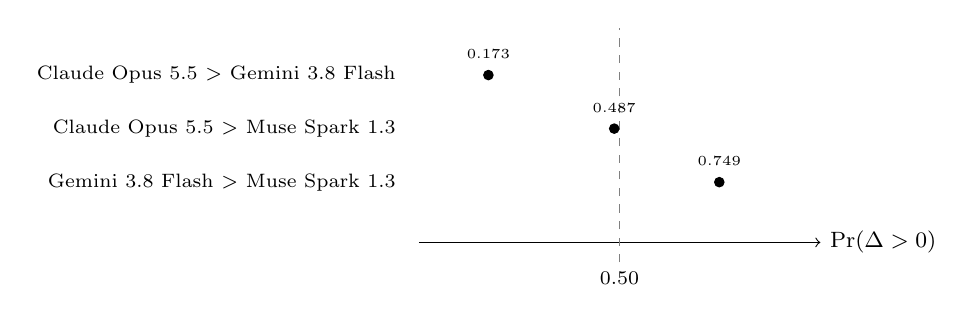
\begin{tikzpicture}[scale=0.85, every node/.style={font=\footnotesize}]
  \draw[->] (0, 0) -- (6, 0) node[right] {$\Pr(\Delta > 0)$};
  \draw[dashed, black!50] (3, -0.3) -- (3, 3.2);
  \node[below, font=\scriptsize] at (3, -0.3) {0.50};
  \node[left, font=\scriptsize] at (-0.2, 2.50) {Claude Opus 5.5 $>$ Gemini 3.8 Flash};
  \draw[fill=black] (1.04, 2.50) circle (2pt);
  \node[above, font=\tiny] at (1.04, 2.60) {0.173};
  \node[left, font=\scriptsize] at (-0.2, 1.70) {Claude Opus 5.5 $>$ Muse Spark 1.3};
  \draw[fill=black] (2.92, 1.70) circle (2pt);
  \node[above, font=\tiny] at (2.92, 1.80) {0.487};
  \node[left, font=\scriptsize] at (-0.2, 0.90) {Gemini 3.8 Flash $>$ Muse Spark 1.3};
  \draw[fill=black] (4.49, 0.90) circle (2pt);
  \node[above, font=\tiny] at (4.49, 1.00) {0.749};
\end{tikzpicture}
\caption{Posterior directional probabilities of pairwise model susceptibility differences. All contrasts span 0.50, indicating inconclusive between-model vulnerability ($\\mathcal{H}_2$).}\label{fig:h2-pairwise-probabilities}
\end{figure}
